% Writeup for MDS
% David Lawrence Miller
% d.l.miller@bath.ac.uk
 
% Started : 22 August 2008
 
\documentclass[a4paper,10pt]{amsart}
 
% Load some packages
\usepackage{times, amsmath, amssymb, amsfonts, url, natbib, bm, rotating}
 
\usepackage{multirow}
\usepackage{graphicx}

% top matter
\title{Multidimensional scaling as a tool for smoothing over complex regions}
\author{David Lawrence Miller}
\email{d.l.miller@bath.ac.uk}
\address{Mathematical Sciences, University of Bath, Bath, United Kingdom}
 
% Shortcuts
% Probability
\newcommand{\prob}[1]{\mathbb{P}\left[ #1 \right]}
% Hovitz-Thompson
\newcommand{\HT}{\hat{\tau}_{HT}}
% Schwarz-Christoffel
\newcommand{\sch}{Schwarz-Christoffel }
% fprime
\newcommand{\fprime}{f^\prime(z)}
% figure reference command
\newcommand{\fig}[1]{\emph{fig.} (\ref{#1})}
% equation reference command
\newcommand{\eqn}[1]{\emph{eqn.} (\ref{#1})}
% phi inverse
\newcommand{\phiinv}{\phi^{-1}}
% use other phi
\renewcommand{\phi}{\varphi}
%transpose
\newcommand{\tr}[1]{#1^{\text{T}}}
% diagonal
\newcommand{\diag}{\text{diag}}



\begin{document}
 
% The abstract
\begin{abstract}
Here.
\end{abstract}
 
 
% New theorem for theorems
\newtheorem{thm}{Theorem}[section]
 
%New theorem for definitions
\newtheorem{defn}{Definition}[section]
 
\maketitle

%\markright{TECH. DETAILS OF SCHWARZ-CHRISTOFFEL MAPPING}

\section{Introduction}

Multidimensional scaling (MDS) or as it is often referred to principle coordinates (PCO) is a method commonly used in multivariate analysis to find a new configuration of points based on the distances between the points (\cite{chatfieldcollins}, p. 187.)

This method provides an obvious framework for the problem of smoothing over a region with a complex boundary. We can use the within-area distances to configure the points in such a way that smoothing does not suffer from leakage.

\section{Multidimensional Scaling}

We first define $d_{ij}$ as the distance between the points $i$ and $j$. How we find $d_{ij}$ is discussed in the next section, for the moment we assume that we know $d_{ij}$.

\cite{diaconis08} gives a clear definition of the algorithm (due to \cite{schoenberg35}) for finding the new locations of points given we know the $d_{ij}$s. 

Taking the unknown new locations and putting them in an $n \times p$ matrix, $X$. Taking $S=X\tr{X}$, and performing an eigen-decomposition we can see that $S=U\Lambda\tr{U}$. So we may now express $S$ as some set of length $n$ vectors (hopfully less than $p$ of them.) We now have that $\tilde{X}=U\Lambda^{1/2}$.

The $d_{ij}$s mentioned above form an $n \times n$ matrix, $D$. We can relate this to $S$, above, by first defining

\begin{equation}
H = I-\frac{1}{n}\mathbf{1}\tr{\mathbf{1}}.
\end{equation}

By pre- and post-multiplying any matrix by $H$ we double centre it (row and column means are 0.) We then obtain\footnote{See \cite{diaconis08} for a simple proof.}:

\begin{equation}
S = -\frac{1}{2}HDH.
\end{equation}

So, in order to obtain a the new configuration of points using MDS (given that we have some set of inter-point distances) we merely need to double centre the matrix of distances and perform an eigen-decomposition.

Multidimensional scaling may be performed in \textsf{R} using the \texttt{cmdscale} function.


\subsection{Finding the within-area distances}

The within-area distances to be fed to MDS are found using a novel algorithm. This works by tracing the inside sides of the polygon and then modifying the path by deleting and replacing portions of the path. Given that there is no direct path within the domain ($\Gamma$, say) between two points ($p_1$ and $p_2$, say), the algorithm proceeds as follows:

\begin{itemize}
\item Create initial path by drawing a line between $p_1$ and $p_2$ (\fig{wdia}, ($i$)) and where they meet the boundary of $\Gamma$ and start the path as the lines from $p_1$, $p_2$ to their first intersection with the boundary of $\Gamma$. Then find the distance between these two intersection points in both directions, along the boundary (\fig{wdia}, ($ii$).) Choose the shorter of these add the paths between $p_1$, $p_2$ and the boundary and this is the starting path(\fig{wdia}, ($iii$).) 
\item Given a triple of vertices, $v_1$, $v_2$, $v_3$ if the line between $v_1$ and $v_3$ is shorter than the path ($v_1$, $v_2$, $v_3$) and the line between $v_1$ and $v_3$ lies inside $\Gamma$ then delete $v_2$ (\fig{wdia}, ($iv$) and ($vi$).) This iterates over the entire path once, deleting all superfluous vertices. 
\item Given a triple of vertices, $v_1$, $v_2$, $v_3$ if the path $v_1$, some subset of the vertices of $\Gamma$, $v_3$ is shorter than the path ($v_1$, $v_2$, $v_3$) then replace $v_2$ with those elements of $\Gamma$ (\fig{wdia}, ($v$)). 
\item We then iterate between steps 2 and 3 until there has been no change from one run to the next (ie. convergence) or there have been too many iterations (\fig{wdia}, ($vi$).)
\end{itemize}

% diagram for finding the shortest path in W
\begin{figure}
\centering
% trim order l b r t
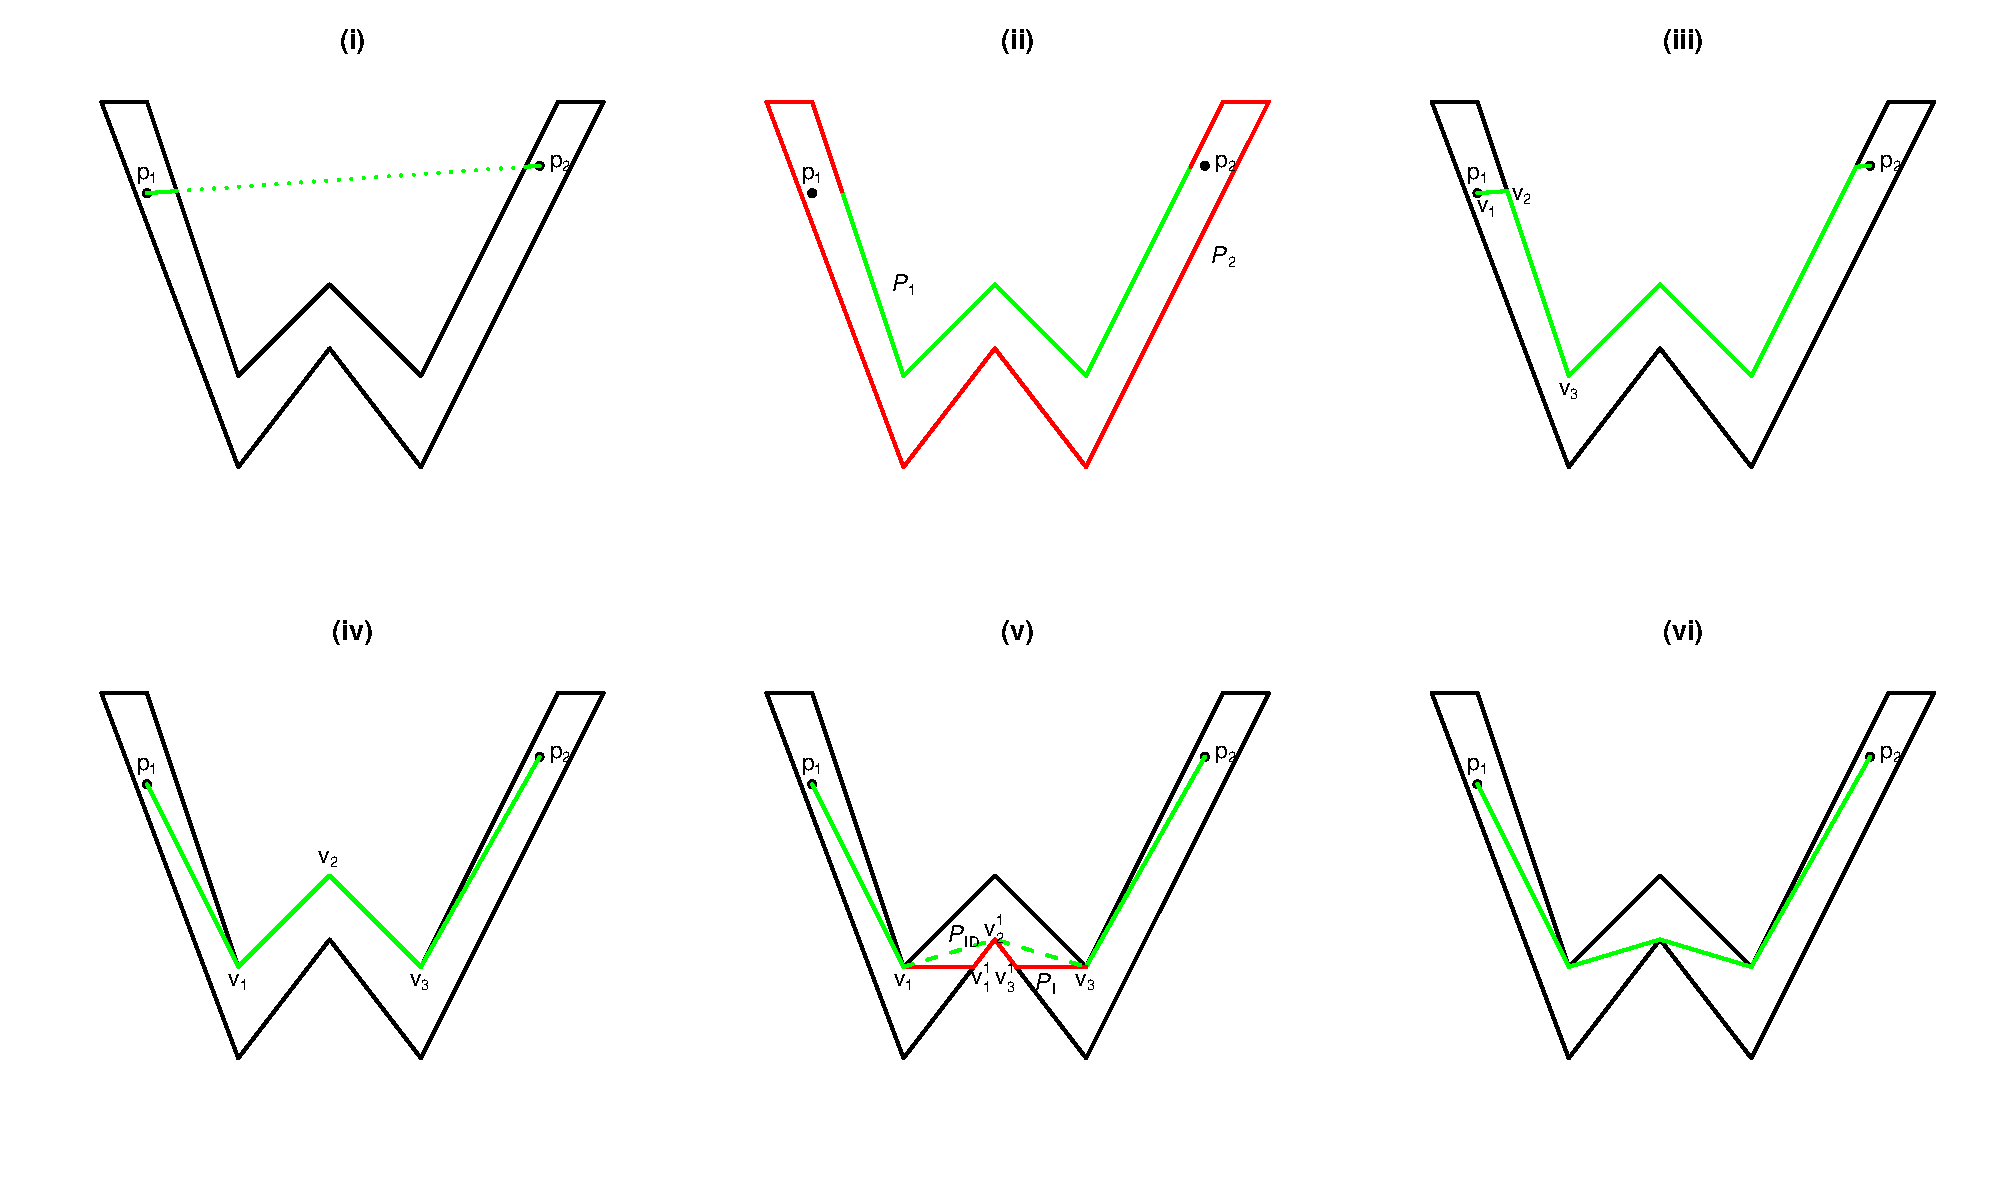
\includegraphics[trim=0in 0in 0in 0in, width=4in]{figs/wdia.pdf} \\
\caption{($i$) to ($vi$) show the path as the algorithm progresses from initial state to final, shortest path. }
\label{wdia}
% generate /phd-smoothing/mds-writeup/figs/distanceexplanation.R
\end{figure}



[[ euclidean distance analysis ]]
\section{Simulation experiment}

Ramsay
mds MSE= 0.002239077 
tprs MSE= 0.0651262 
soap MSE= 0.001455530 


wt2
mds=0.1291663
tprs=0.0760142
soap=0.02217734



do plots of vis.gam() with too.far set low and overlay of points

boxplots



\section{Conclusions}


\bibliographystyle{plainnat}
\bibliography{mds-refs}

\end{document}
